\documentclass[/home/greg/Thesis/main/main.tex]{subfiles}

\begin{document}

\graphicspath{{/home/greg/Neutron_star_modelling/LyneSwitchingAnalytic/img/}}

 \newcommand{\dST}{\Delta\fdot_{T}}
\renewcommand{\tref}{t_{\textrm{R}}}

\newcommand{\two}[2]{
\left\{
\begin{array}{cc}
#1  &t \in A \\
#2& t \in B
\end{array}•
\right.}

%\subsection{Introduction}

\section{Analytic description of the two state switching}
The two state switching model is defined by two distinct spindown values and the
durations that the system spends at each value. The spindown follows a square
wave pattern, numerically integrating this with appropriate initial values yields the
frequency and phase. This basic model was investigated by \citet{Lyne2010} and
\citet{Perrara2014} by fitting and removing a Taylor expansion to the phase to
produce the timing residual of such a system. 
It was found by \citet{Lyne2010} that this deterministic
system must be modified by the introduction of some randomness to match 
observed residuals. 

In this section we will consider only the deterministic system and develop an
analytic result matching the numerical result. This analytic result allows us
to better understand the simple two-state switching model.

First, let us define two periods labelled by $A$ and $B$, these refer to the
two states which the system switches between. If the system spends time $t_{A}$
in state A, and $t_{B}$ in state B then repeats, we can define the total
duration of a single cycle and a ratio between the two states as
\begin{align}
    T = t_{A} + t_{B}  &&& R = t_{A}/t_{B}.
\end{align}
In each period the spin-down rate is a constant given by $\fddot_{X}$ where $X \in [A, B]$.
Therefore during each period the phase evolution will be described by a Taylor
expansion such as \eqref{eqn: taylor}. Let us define the parameters of the Taylor
expansion 
in each period as $\bl_{X}=[\phi_{X}, \f_{X}, \fdot_{X}]$; then we can 
write a time dependent set of parameters as
\begin{align}
\bl(t) = \two{\bl_{A}}{\bl_{B}} 
\label{eqn: lambda t}
\end{align}
Similar expression can be written for each of the components (e.g. $f(t)$).
We also need to define the reference time for each period: we choose to set this
halfway through the respective period. The full time-dependant
reference time can then be written
\begin{align}
\tref(t) = \two{\frac{T}{2}R}{\frac{T}{2}(R+1)}
\end{align}
Having defined the time-dependant parameters and reference time, the global
phase model valid from $[0, T]$ is given by
\begin{equation}
\Phi(t; \bl(t), \tref(t)) = \phi(t) + 2\pi\left(\f(t)(t-\tref(t)) + \frac{\fdot(t)}{2}\left(t-\tref(t)\right)^{2}\right)
\label{eqn: phase switched}
\end{equation}

\subsection{Calculating the phase residual} The phase residual $\Delta\Phi(t)$ is
the difference between the actual phase of the pulsar and a best fit global
Taylor expansion. The term global distinguishes a single Taylor
expansion over the entire duration from the local templates used to
model the phase of model. By \emph{best fit} we refer to the global template which minimises
the phase residual. usually this is done using a least-squares method.

First we ignore the best-fit requirement and define only how to analytically
calculate the phase residual. Explicitly the phase residual is
defined as
\begin{equation}
\Delta\Phi(t) = \Phi(t; \bl(t), \tref(t)) - \Phi(t; \bl_{G}(t), \tref(t)),
\end{equation}

The term $\Phi(t; \bl(t), \tref(t))$ describes the phase evolution in the
switched spindown model (eqn. \eqref{eqn: phase switched}), while $\Phi(t; \bl_{G}(t), \tref(t))$ refers to the
phase of the global template. 

The global template is defined by a single set of
coefficients and corresponding reference time. However, if want to describe the
system such that at a given time
the model and global template refer to the same reference times $\tref(t)$, we
can explicitly break up the global template into segments coinciding with
those of the switching model. In this way the global reference time is still
defined by a single set of coefficients and reference time, but these are 
translated to the relevant reference times $\tref(t)$ such that all the individual
segments lie on the same global template. This allows the phase residual to be written as
\begin{equation}
\Delta\Phi(t; \bdl(t), \tref(t)) = \Delta\phi(t) + 2\pi\left( \Delta\f(t)(t-\tref(t)) + \frac{\Delta\fdot(t)}{2}\left(t-\tref(t)\right)^{2}\right)
\label{eqn: general phase residual}
\end{equation}
where  
\begin{equation}
\bdl(t) = \bl(t) - \bl_{G}(t) = \left\{
\begin{array}{cc}
\bdl_{A} & t \in A \\
\bdl_{B} & t \in B
\end{array}•
\right. .
\end{equation}
%$The components are $\bdl_{x}=[\Delta\phi_{x}, \Delta\f_{x}, \Delta\fdot_{x}]$
%where $x \in [A, B]$.
Writing the phase residual in such a way removes the requirement to consider
the monotonic spindown. Instead, we can focus on the difference between the
model and the global template.  

\subsection{Modelling the two-state switching}
Now we are ready to start modelling the two state switching. From equation 
\eqref{eqn: lambda t} we can write the spin-down rate as
\begin{equation}
\fdot(t) = \two{\fdot_{A}}{\fdot_{B}}.
\end{equation}
Now we rewrite this expression by defining a time-dependant spin-down offset
about the global template:
\begin{equation}
\fdot(t) = \fdot_{G} + \Delta\fdot(t),
\end{equation}
here we assume $\fddot_{G}=0$ such that $\fdot_{G}$ is a constant. Then we have
implicitly defined the time-dependant offset as
\begin{equation}
\Delta \fdot(t) = \two{\dSA}{\dSB} .
\end{equation}
with $\Delta \fdot_{X} = \fdot_{X} - \fdot_{G}$. In figure~\ref{fig: F1} we 
illustrate the setup over a single cycle of $A$ and $B$.
\begin{figure}[htb]
\centering
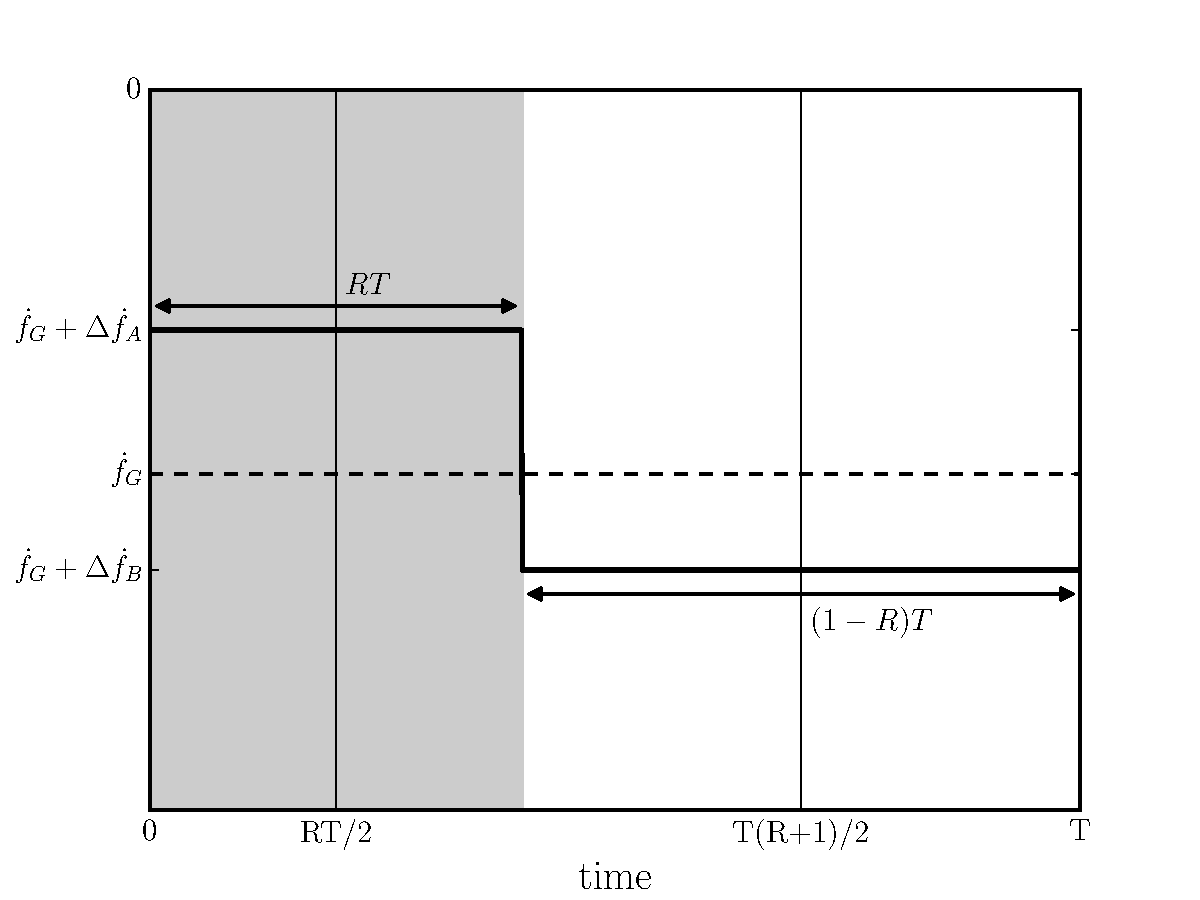
\includegraphics[width=.6\textwidth]{F1}
\caption{Illustration of the switched spindown model over one cycle.}
\label{fig: F1}
\end{figure}

\FloatBarrier
\subsection{Calculating the best fit for the two-state switching}
We now need to define what we mean by the `best fit'. For observational data
and the numerical models of \citet{Lyne2010} and \citet{Perrera2014}, this
resulted from a least-squares fitting procedure. While we could replicate
this process analytically, we can also proceed by a more intuitive method. 

The
phase residual of equation \eqref{eqn: general phase residual} is given for a 
single cycle, in reality we want to calculate the best fit over several cycles.
Therefore we define the best fit model as the set of coefficients $[\bdl_{A}, \bdl_{B}]$
which minimises $\Delta\Phi(t)$ over several cycles. The free parameters of the
model are the jump in spin-down which occurs between the two segments, and the
relative times spent in each segment. This leaves the frequency and phase
offsets in each segment and one of the spin-down offsets to be calculated. Note
only one spin-down value is required since the other can be set from the jump
in spin-down. We can constrain these unknown parameters by setting up 
5 simultaneous
equations reflecting our choice of best fit.
In each case the property is given and the
equation resulting from applying equation~\eqref{eqn: general phase residual}
is then given.

\begin{itemize}

\item \emph{No accumulations of phase:} In order for $\Delta\Phi$ to remain
    bounded and not grow with each cycle we require that the phase offset at
    the beginning of a cycle be equal to that at the end:

\begin{align}
\Delta\Phi(0) & = \Delta\Phi(T) 
\end{align}•
\begin{equation}
0  = \dPB - \dPA+ \pi\left(T\left(\dFA R + \dFB (1-R)\right) + \frac{T^{2}}{4}\left(\dSB (1-R)^{2} - \dSA R^{2}\right)\right)
\end{equation}•

\item\emph{Smooth phase at the interface:} The interface between the two
    segments occurs at $t_{A} = RT$. For the best fit, the phase and hence
    $\Delta\Phi(t)$ should be smooth at this point
\begin{align}
\lim_{t\rightarrow t_{A}^{-}}\Delta\Phi(t) = \lim_{t\rightarrow t_{A}^{+}}\Delta\Phi(t)
\end{align}•
\begin{equation}
0 = \dPB - \dPA + \pi\left(-T\left(\dFA R + \dFB (1-R)\right) + \frac{T}{4}\left(\dSB (1-R)^{2} - \dSA R^{2}\right)\right)
\end{equation}
In addition, for the best fit the phase offset in each segment must carry opposite signs if the total phase accumulation 
is to vanish. This must mean that the phase offset at the interface between the two segments is zero such that
\begin{align}
\lim_{t\rightarrow t_{A}^{-}}\Delta\Phi(t) = \lim_{t\rightarrow t_{A}^{+}}\Delta\Phi(t)=0
\end{align}
Either of these relation can be used, from the first we have
\begin{align}
\Rightarrow 0 & = \Delta\phi_{A} + \pi\left(\dFA RT + \dSA \frac{R^{2}T^{2}}{4}\right)
\end{align}•


\item\emph{No accumulation of frequency:} In a similar manner to the phase, we expect that

\begin{align}
\frac{d\Delta\Phi(0)}{dt} & = \frac{d\Delta\Phi(T)}{dt} 
\end{align}•
\begin{equation}
0 = \dFB - \dFA + \frac{T}{2}\left(\dSA T+ \dSB (1-R)\right)
\end{equation}

\item\emph{Smooth frequency at the interface:} 
\begin{align}
\lim_{t\rightarrow t_{A}^{-}}\frac{d\Delta\Phi(t)}{dt} = \lim_{t\rightarrow t_{A}^{+}}\frac{d\Delta\Phi(t)}{dt}
\end{align}
\begin{equation}
0 = \dFB - \dFA - \frac{T}{2}\left(\dSA R + \dSB (1-R)\right)
\end{equation}
\end{itemize}•

Working through this system of equations we end up with the following set of
parameters for residual of the best fit
\begin{align}
\Delta\fdot(t) &= \two{\dSA}{-\frac{R}{1-R}\dSA} & 
\Delta\f(t) &= 0 &
\Delta\phi(t) = \two{-\frac{\pi}{4} \dSA T^{2}R^{2}}{\frac{\pi}{4}\dSA T^{2}(R-R^{2})} &
\end{align}
Then the phase residual can be written as
\begin{equation}
\Delta\Phi(t) =\pi\dSA \two{
    -\left(RT/2\right)^{2} + \left(t-(RT/2)\right)^{2}}
    {\left(T/2\right)^{2}(R-R^{2}) - \frac{R}{1-R}\left(t-\frac{T}{2}\left(R+1\right)\right)^{2}}
\label{eqn: phase residual}
\end{equation}

We can make this slightly more general by defining the total difference in
spindown between two states as $\Delta\fdot_{T} = |\dSA - \dSB|$ such that the phase
residual can be written as
\begin{equation} 
    \Delta\Phi(t; \Delta\fdot_{T}, t_{A}, R) = \pi\Delta\fdot_{T}\two{
        (1-R)t(t-RT)
         }
        {
       -R(t-T)(t-RT)
        }
\label{eqn: full phase residual}
\end{equation}•
This gives the best phase residual in a single cycle for $t$ is bound by $[0, T]$ when fitting
through many such cycles. Note that 
this is not the same as the best fit phase residual over a single cycle. 

In figure \ref{fig: Lyne analytic illustration} we illustrate the critical points of the
phase residual during a single cycle. Note that when $R\ne1/2$ the radius of
curvature of the maxima and minima will differ.
\begin{figure}[ht]
    \centering
    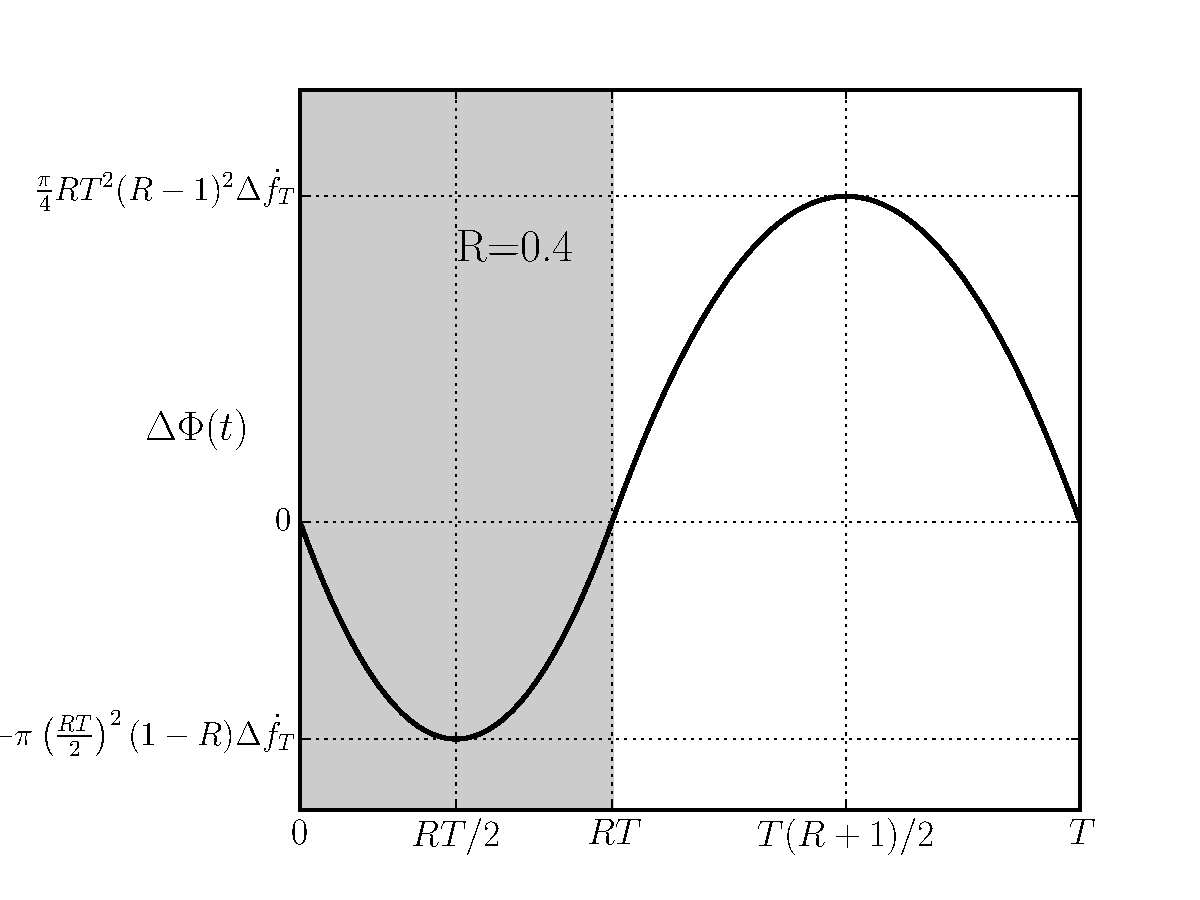
\includegraphics[width=.75\textwidth]{DP.pdf}
    \caption{Phase residual over a single cycle, due to our choice of the best
             fit this pattern will repeat for each cycle}
    \label{fig: Lyne analytic illustration}
\end{figure}

\subsection{Extending the model to an arbitrary number of cycles} The phase
residual and hence mismatch calculated above consider only fitting to 
one single cycle of switching.  Since we calculated the best fit over several cycles, we know that
in any given cycle the residual will be the same, provided that an integer number
of cycles is fitted. Therefore we can extend equation
\eqref{eqn: full phase residual}
to an any arbitrary number of cycles by
defining~$\tilde{t}= t \mod T$. The phase residual is then 
\begin{equation} 
    \Delta\Phi(t; \Delta\fdot_{T}, R) = \pi\Delta\fdot_{T}\two{
        (1-R)\tilde{t}(\tilde{t}-RT)
         }
        {
        -R(\tilde{t}-T)(\tilde{t}-RT)
        }
\label{eqn: arbitary full phase residual}
\end{equation}•
with the assumption that the initial cycle starts at $t=0$. 
Note that this is \emph{not} a fully general model since it assumed we have
fitted to an integer number of cycles. If some fraction of a cycle existed
at the start and end of the observation then the residual may be skewed by
favouring one state or the other. Nevertheless, this method should illustrate
the essential features of the residual in the limit that enough full cycles
are observed not to favour one or the other.

In figure \ref{fig: Lyne analytic verification} we have plotted the analytic 
prediction for the phase residual over several cycles. This is compared with
a numerical result obtained in the manor of \citet{Lyne2010}: starting by defining
a time dependant spin-down, we integrate twice to get the phase, then fit and
subtract a timing model to get the residual. 
\begin{figure}[ht]
    \centering
    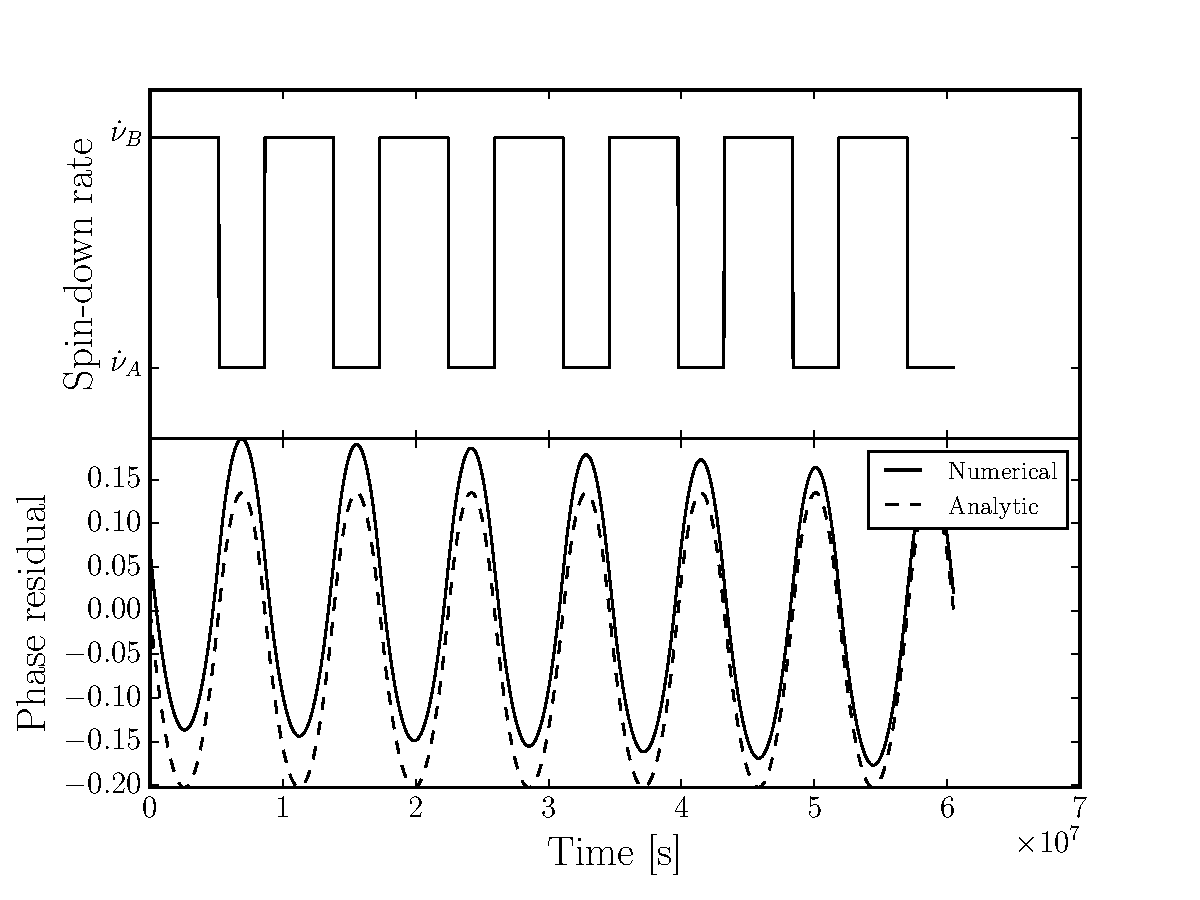
\includegraphics[width=.75\textwidth]{verification_example.pdf}
    \caption{}
    \label{fig: Phase residual}
\end{figure}

\FloatBarrier
\subsection{Verifying the model}

\textcolor{red}{This section is broken since the fitting does not appear to be
sufficiently good to do this!}

Having an analytic expression for the phase residual means observational results
could be tested to see if they agree with this model. Ideally we would like to
apply this to the results in \citet{Lyne2010}. This could help quantify how
well the observed timing residuals can be explained by a two-state switching model
compared to a random walk model. Two methods are presented which could easily
be applied to data.

\subsubsection{Magnitude of peaks}
Firstly if we divide the absolute values of the phase residuals at the extrema, which occur at the reference
times in this parameterisation, then we have
\begin{equation}
    \left|\frac{\Delta\Phi\left(RT/2\right)}{\Delta\Phi\left(T(R+1)/2\right)}\right|
    = \frac{\frac{\pi}{4}\Delta\dot{f_{T}} T^{2}(R-R^{2})}{\frac{\pi}{4}\Delta\dot{f_{T}} T^{2}(R-1)^{2}}
= \frac{R}{R-1}
\end{equation}
This is exactly the ratio of the durations of the two segments.  


\subsection{Radii of curvature}
\citet{Hobbs2010} found that `the residuals are generally asymmetric in that the radii 
of curvature of local maxima and minima are often consistently different'. The radii of curvature
for a curve $y(x)$ is given by 
\begin{equation}
    r(x) = \frac{\left(1 + y'(x)\right)^{3/2}}{y''(x)}
\end{equation}
For equation~\eqref{eqn: phase residual}  the radii of curvature at the extrema are then
\begin{align}
    r\left(RT/2\right) = \frac{-R}{2\pi\Delta{\dot{f}_{T}}(R-1)} && 
    r\left(T(R+1)/2\right) =  \frac{-1}{2\pi\Delta{\dot{f}_{T}}} 
\end{align}
For the observation that the radii of curvature to be different in this model we then require $R\ne 1/2$. 
This can also be measured from the timing residual.

\subsection{Testing agreement}
We can verify that our analytic model approximates the phase residual magnitudes
by comparing with a numeric calculation. That is, we reproduce the model of
\citet{Lyne2010} by generating a square-wave for the spin-down, integrating
twice to get the phase, fitting and removing a Taylor series yeilds the 
phase residual. This was done for several cycles of switching and in figure
\ref{fig: compare analytic numeric two state} we illustrate how the magnitude
of the phase-residual varies for the numeric calculation and the analytic
preduction of \eqref{eqn: full phase residual}. 

\begin{figure}
    \centering
    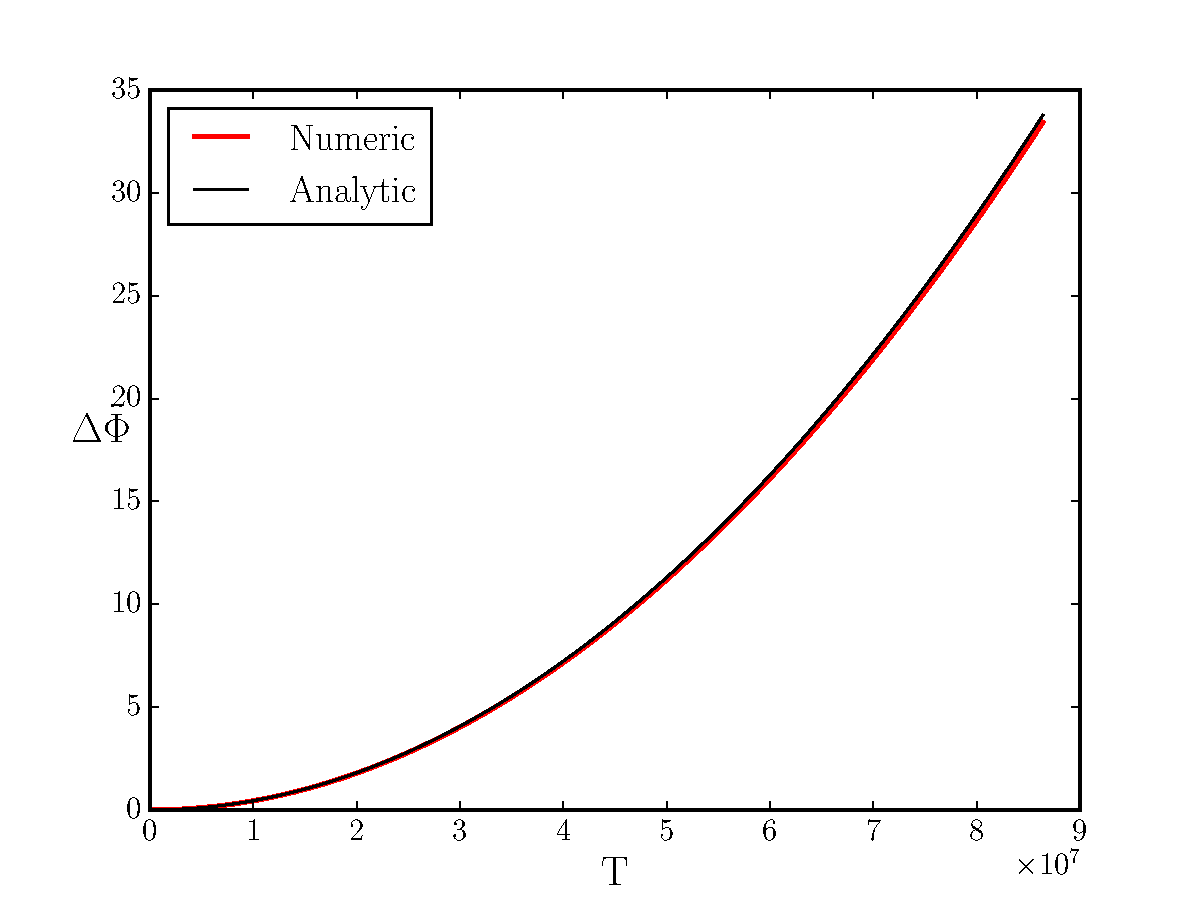
\includegraphics[width=.5\textwidth]{TestingMagnitude}
    \caption{}
    \label{fig: compare analytic numeric two state}
\end{figure}

\end{document}
